\documentclass[11pt]{article}

\usepackage{graphicx}
\usepackage[top=25mm, bottom=25mm, left=25mm, right=25mm, a4paper]{geometry}
\usepackage{amsmath}
\usepackage{enumitem}
\usepackage{float}
\usepackage{fancyhdr}
\usepackage{booktabs}
\usepackage{tikz}
\usepackage{steinmetz}
\usepackage{pgfplots}

\pagestyle{fancy}
\fancyhf{}
\fancyhead[R]{Baturay Kafkas - 2240357068 - Electrical \& Electronics Engineering}

\rfoot{\thepage}
\renewcommand{\headrulewidth}{0pt} 
\renewcommand{\footrulewidth}{0pt}
\sloppy

\begin{document}

\begin{center}
\large
\textbf{ELE214 - Electronics Laboratory I Preliminary Work 2}
\end{center}

\section{Questions}

\begin{enumerate}[leftmargin=*,label=\textbf{\arabic*.}]

\item Plot the typical Zener diode characteristics and specify the breakdown voltage $V_z$, the minimum Zener current $I_{z,\text{ min}}$, and the threshold voltage $V_o$. 

\begin{figure}[H]
    \centering
    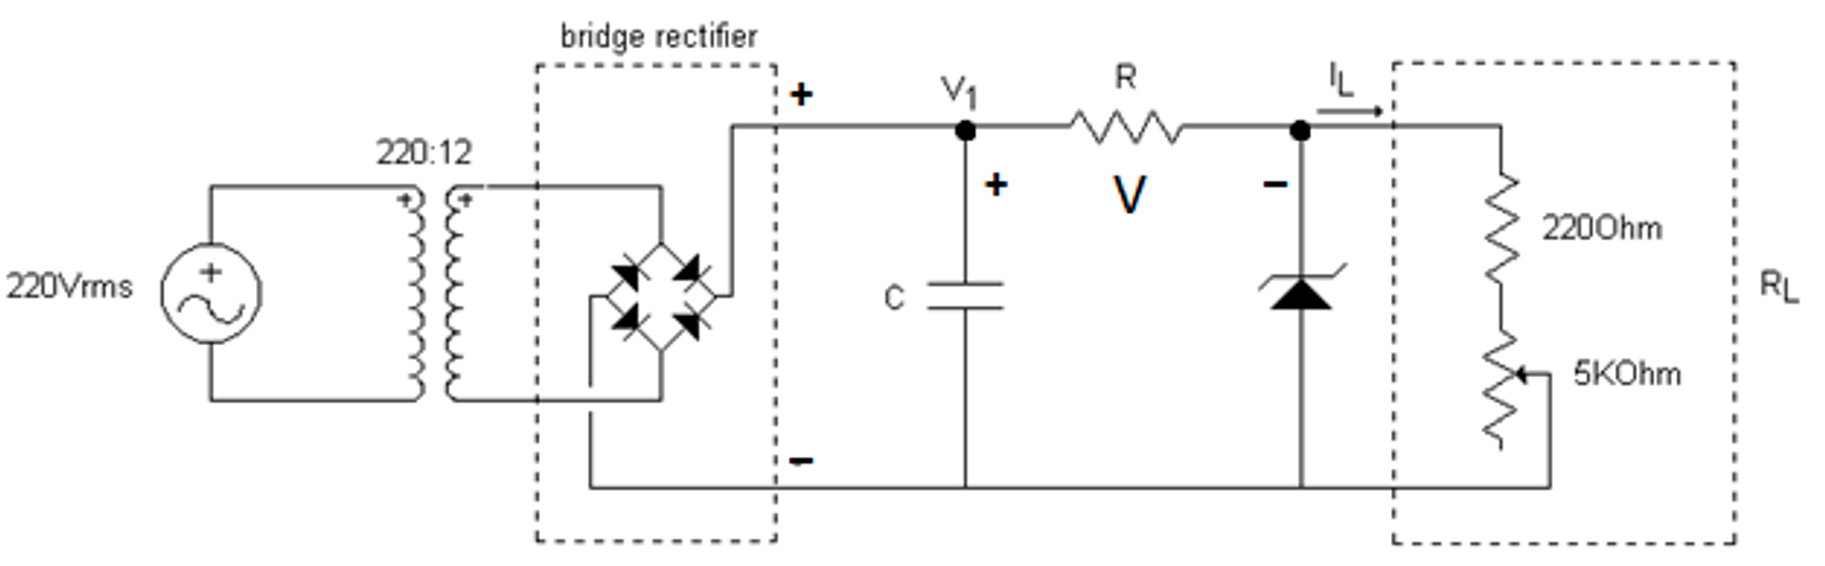
\includegraphics[width=0.9\linewidth]{lvGvfEIkof.png}
    
    \textit{Circuit 1}
\end{figure}

The following questions are related to the regulator circuit shown in the figure. Zener diode characteristics are: $V_z= 7.5\text{ V},\: I_{z,\text{ min}}= 20\text{ mA and } P_{z,\text{ max}}=500\text{ mW}$.

\item Assume that ripple voltage is zero and calculate the voltage denoted as $V_1$.

\item For load resistance $R_L$ varying between $220$ and $5220$ ohms, calculate maximum $(I_{L,\text{ max}})$ and minimum $(I_{L,\text{ min}})$ load currents flows through Zener diode. 

\item Assuming the Zener diode is dissipating its maximum power, load current values are as calculated in part $3$, and load voltage ($V_L$) is constant at $7.5$ V, what should be the value of the resistor $R$?

\item Assuming that $R=150$ $\Omega$, calculate the maximum value of $V_1$ that will cause the Zener diode to be burnt. 

\end{enumerate}

\textbf{Experimental Work (Simulation of 2-3)}

\begin{enumerate}[leftmargin=*,label=\textbf{\arabic*.}]

\item With the available components on the desk, design and set up a circuit to obtain the characteristic curve of a Zener diode on the oscilloscope. Plot the curve indicating critical points.

\item Set up the circuit in the figure for $R=150$ $\Omega,\: C=100\:\mu$F. For maximum and minimum $R_L$, measure the maximum and minimum values of $I_L$ and $V_L$.

\item Connect a $R_p=1\:k\Omega$ potentiometer in series with the resistor $R$. Varying the $R_p$, determine the values of branch voltage $V_\text{max}$, and $V_\text{min}$. For $V=V_\text{max}$, measure $V_{L,\text{ min}}$ and $V_{L,\text{ max}}$ by changing $R_L$. For $V=V_\text{min}$, measure $V_{L,\text{ min}}$ and $V_{L,\text{ max}}$ by changing $R_L$.

\end{enumerate}

\newpage

\section{Answers}

\begin{enumerate}[leftmargin=*,label=\textbf{\arabic*.}]

\item The graph is given below.

\begin{minipage}{0.45\textwidth}
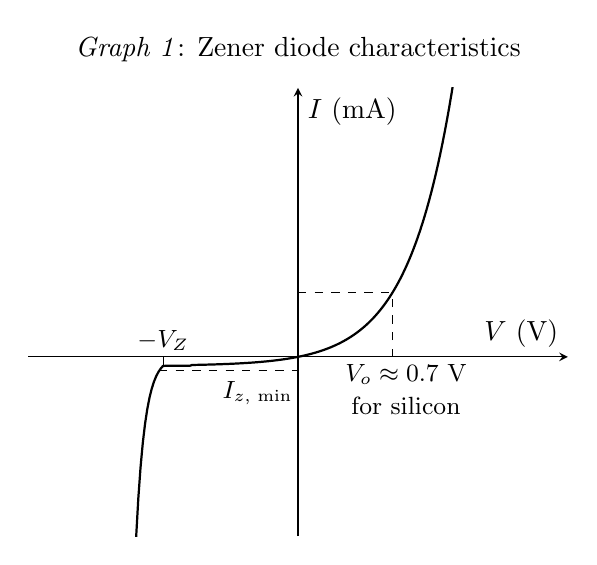
\begin{tikzpicture}
\begin{axis}[
    xlabel={$V$ (V)},
    ylabel={$I$ (mA)},
    xmin=-2, xmax=2,
    ymin=-20, ymax=30,
    axis lines=middle,
    xtick=\empty,
    ytick=\empty,
    title={\textit{Graph 1}: Zener diode characteristics}
]

% Silicon diode
\addplot[
    domain=-1.3:2,
    samples=200,
    thick
]
{ x < -0.8 ? (x < -1 ? 1/e^15*(-e^(-15*x)) : e^(30*x)-1) : exp(3*x) - 1 };

\draw[dashed] (axis cs: 0.7, 0) -- (axis cs: 0.7, 7.166) (axis cs: 0, 7.166) -- (axis cs: 0.7, 7.166) (axis cs: -1, 0) -- (axis cs: -1,-1) (axis cs: -1.03, -1.5) -- (axis cs: 0,-1.5);

\node at (axis cs: 0.8, -2) {\small $V_{o}\approx 0.7$ V };
\node at (axis cs: 0.8, -5.5) {\small for silicon};
\node at (axis cs: -1, 1.8) {\small $-V_Z$};
\node at (axis cs: -0.3, -4) {\small $I_{z,\text{ min}}$};

\end{axis}
\end{tikzpicture}
\end{minipage}\hfill\begin{minipage}{0.45\textwidth}
The Zener diode is essentially a silicon diode intentionally modified to cause a breakdown at a specific voltage $-V_Z$, and it provides a constant voltage within a certain range of current in the reverse bias mode.
\end{minipage}

\item The peak voltage across the secondary side: $V_m=220\cdot\dfrac{12}{220}\sqrt2=12\sqrt2$ V. If we assume the ripple voltage is $0$, then
\[V_1=V_m-2V_{D,\text{ ON}}=12\sqrt2-2\cdot0.7\approx15.57\text{ V}.\]

\item For $I_{L,\text{ min}}$, the load resistance should be high, and vice versa for $I_{L,\text{ max}}$.
\[I_{L,\text{ min}}=\frac{V_Z}{R_{L,\text{ max}}}=\frac{7.5}{5220}=1.44\text{ mA},\qquad I_{L,\text{ max}}=\frac{V_Z}{R_{L,\text{ max}}}=\frac{7.5}{220}=34.10\text{ mA}.\]

\item The voltage across the resistor $R$:
\[V_R=V=V_1-V_Z=15.57-7.5=8.07\text{ V}.\]

For the Zener diode to dissipate maximum power,
\[I_{Z,\text{ max}}=\frac{P_{z,\text{ max}}}{V_Z}=\frac{0.5}{7.5}=66.67\text{ mA}.\]

By KCL,
\[I_{Z,\text{ max}}=I_{R,\text{ max}}-I_{L,\text{ min}}\implies I_{R,\text{ max}}=I_{Z,\text{ max}}+I_{L,\text{ min}},\]
\[I_{R,\text{ max}}=66.67 + 1.44 = 68.11 \text{ mA}\implies R_\text{min}=\frac{V}{I_{R,\text{ max}}}=\frac{8.07}{68.1\times10^{-3}}=118.48\:\Omega.\]

\item The condition for the Zener diode to burn: $I_Z>I_{Z,\text{ max}}$. By Ohm's law,
\[V_{1,\text{ burn}}-V_Z=I_{R,\text{ max}}\cdot R=\left(I_{Z,\text{ max}}+I_{L,\text{ min}}\right)\cdot R,\]
\[V_{1,\text{ burn}}=\left(66.67+1.44\right)\cdot 150+7.5=17.72\text{ V}.\]

\end{enumerate}

\newpage

\textbf{Simulation}

\begin{enumerate}[leftmargin=*,label=\textbf{\arabic*.}]
\setcounter{enumi}{1}

\item The circuit:

\begin{figure}[H]
    \centering
    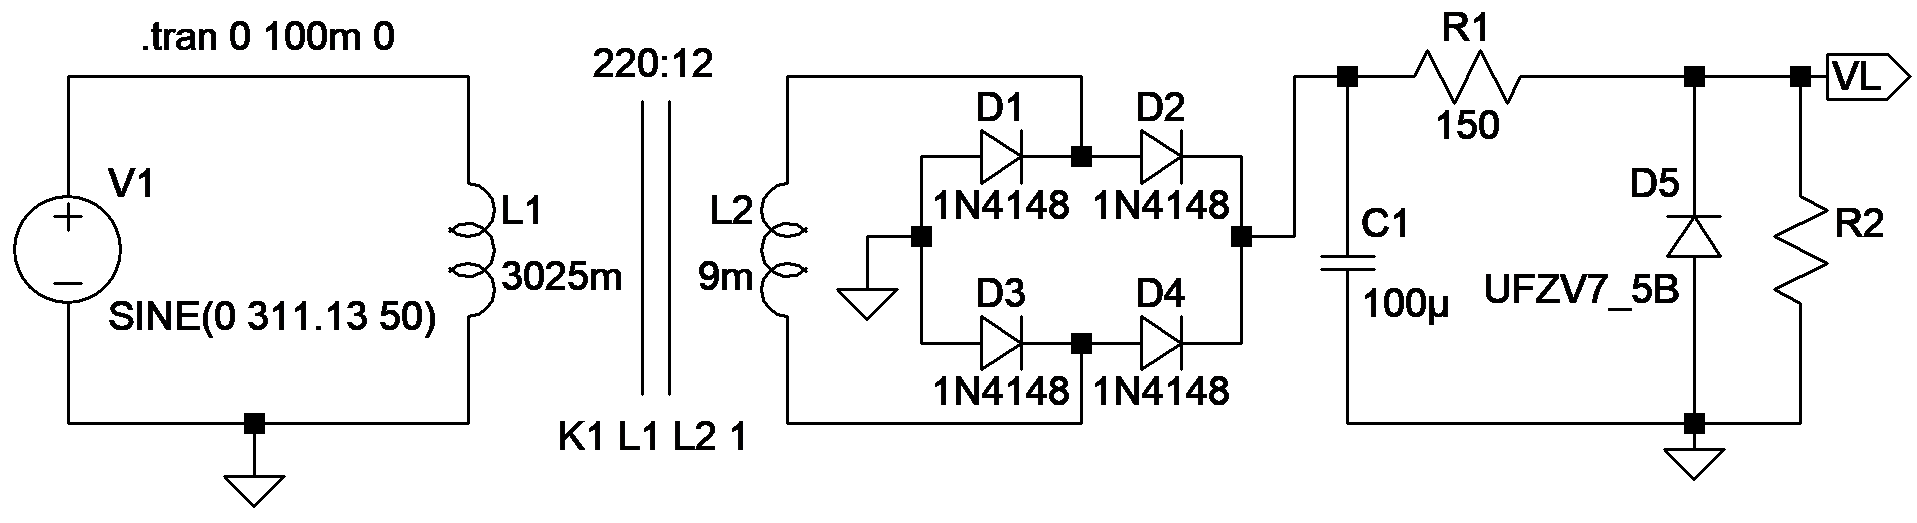
\includegraphics[width=1\linewidth]{q2.png}
    
    \vspace{-1em}
    
    \textit{Circuit 2}
\end{figure}

The minimum and maximum values:

\vspace{0.5em}

\begin{minipage}{0.48\textwidth}
\centering
For $R_L=220\:\Omega$,
\begin{figure}[H]
    \centering
    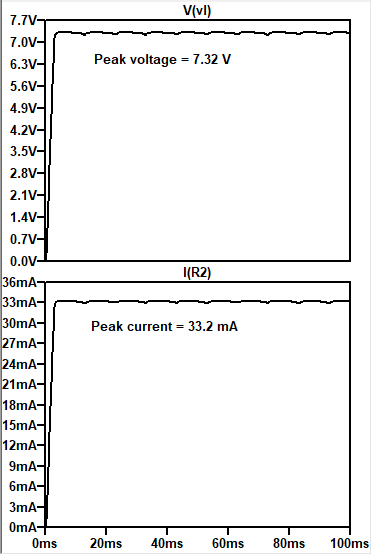
\includegraphics[width=0.85\linewidth]{LTspice_QiEcfYIFud.png}

    \textit{Graphs 2 \& 3:} $V_L$ \textit{and} $I_{R_L}$
\end{figure}
\end{minipage}\vrule\hfill\begin{minipage}{0.48\textwidth}
\centering
For $R_L=5220\:\Omega$,
\begin{figure}[H]
    \centering
    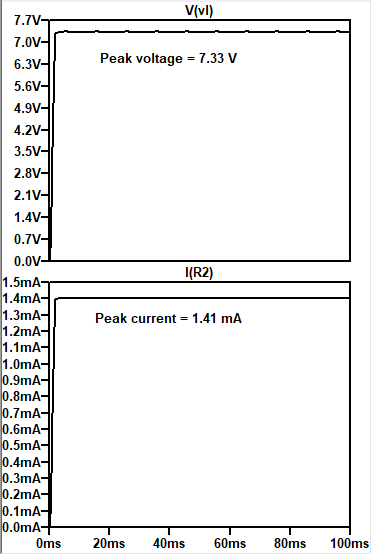
\includegraphics[width=0.85\linewidth]{LTspice_1aLbfGvx8C.png}

    \textit{Graphs 4 \& 5:} $V_L$ \textit{and} $I_{R_L}$
\end{figure}
\end{minipage}

\vspace{1em}

\item The circuit for $R_L=220\:\Omega$:

\vspace{-1em}

\begin{figure}[H]
    \centering
    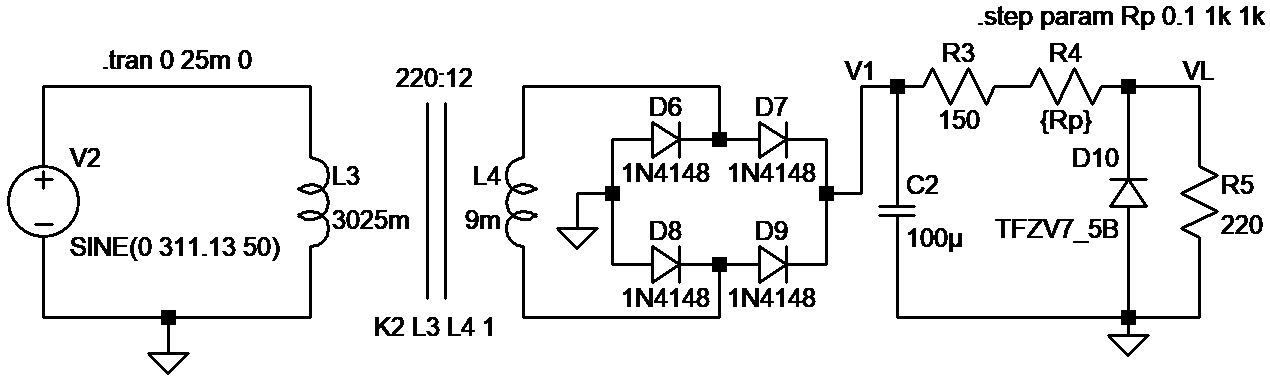
\includegraphics[width=1\linewidth]{q3_2.png}
    \textit{Circuit 3}
\end{figure}

\begin{figure}[H]
    \centering
    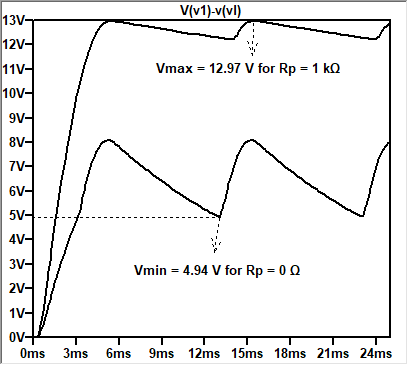
\includegraphics[width=0.5\linewidth]{LTspice_fXf8gch2Mv.png}
    
    \textit{Graph 6: Circuit 3 graphed}
\end{figure}

Note that the value of $V_\text{min}$ is almost identical to the one for when $R_L=5220\:\Omega$. Therefore, take $V_\text{min}=4.94$ V.

For $V=V_\text{max}$, the circuit and its graph are given below.

\begin{figure}[H]
    \centering
    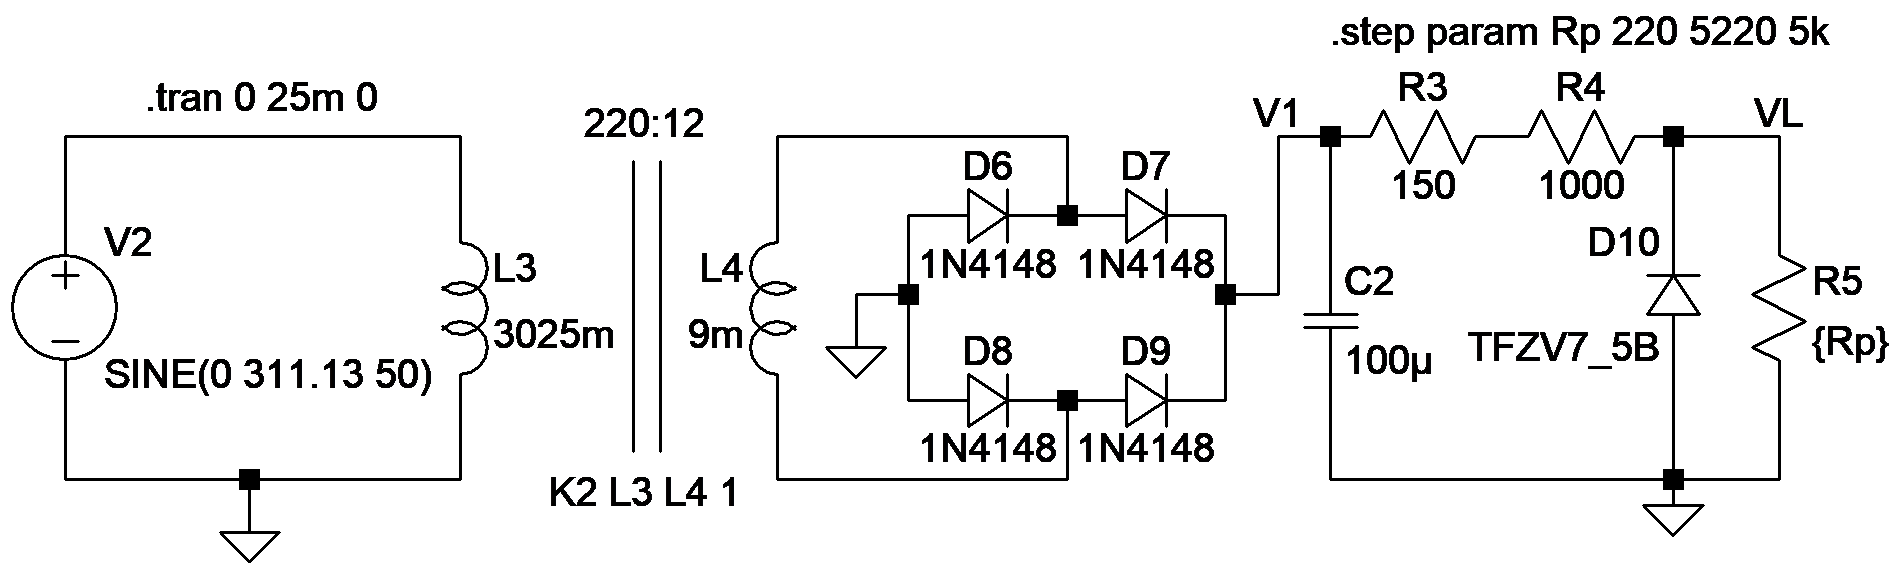
\includegraphics[width=1\linewidth]{q3_3.png}
    \textit{Circuit 4}
\end{figure}

\begin{figure}[H]
    \centering
    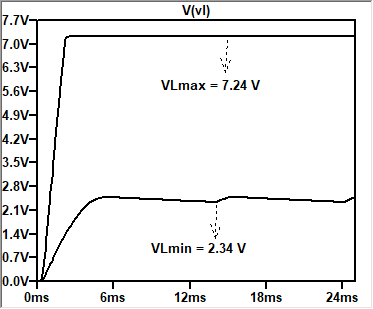
\includegraphics[width=0.5\linewidth]{LTspice_t6JzseRcuQ.png}
    
    \textit{Graph 7: Circuit 4 graphed}
\end{figure}

$V_{L, \text{ min}} = 2.34$ V obtained for $R_L = 220\:\Omega$ and $V_{L, \text{ max}} = 7.24$ V obtained for $R_L = 5220\:\Omega$.

For $V=V_\text{min}$, the circuit and its graph are given below.

\begin{figure}[H]
    \centering
    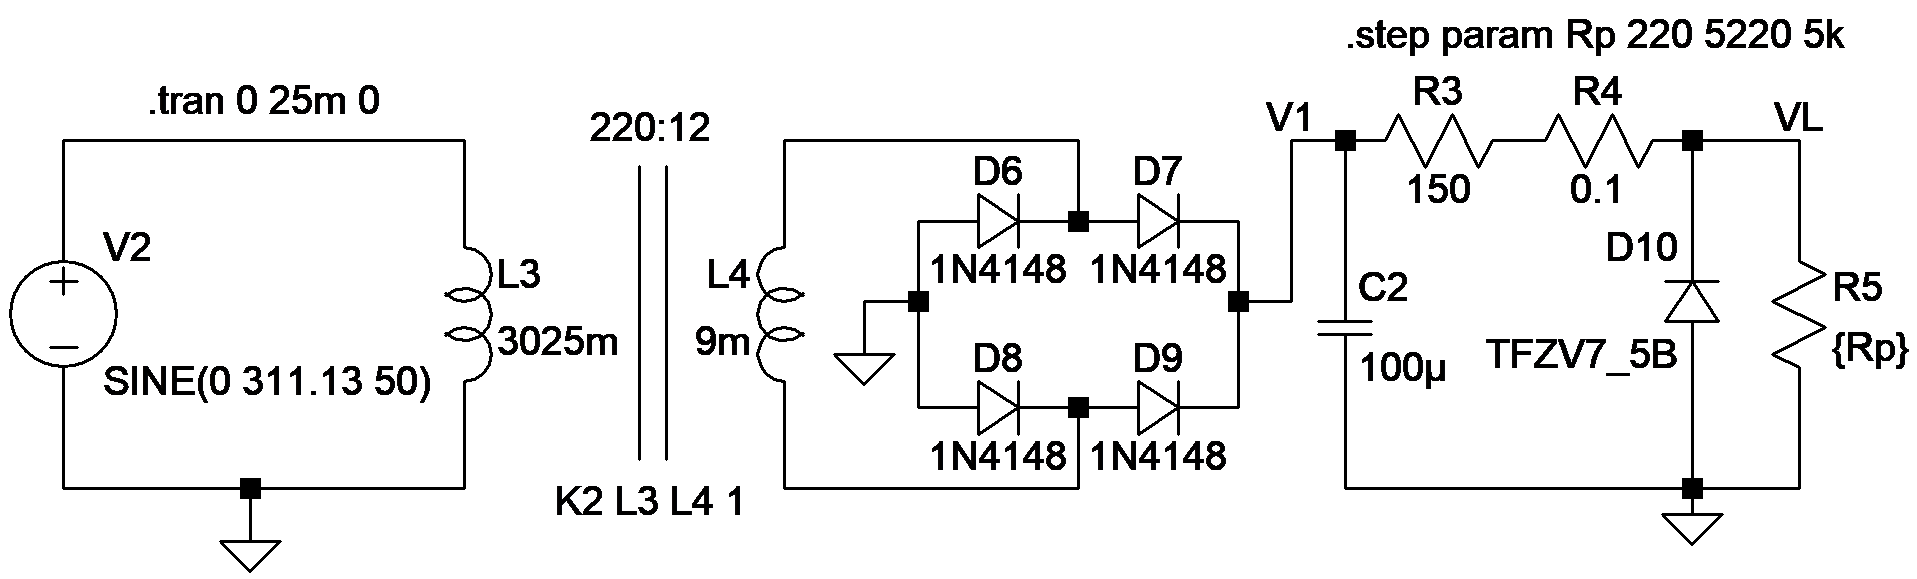
\includegraphics[width=1\linewidth]{q3_4.png}
    \textit{Circuit 5}
\end{figure}

\begin{figure}[h]
    \centering
    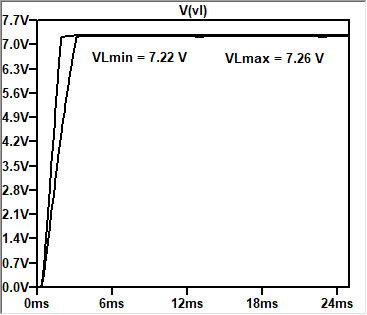
\includegraphics[width=0.5\linewidth]{LTspice_BBiuRLniIr.png}

    \textit{Graph 8: Circuit 5 graphed}
\end{figure}

$V_{L, \text{ min}} = 7.22$ V obtained for $R_L = 220\:\Omega$ and $V_{L, \text{ max}} = 7.26$ V obtained for $R_L = 5220\:\Omega$.

\end{enumerate}

\end{document}